%"runningheads" enables:
%  - page number on page 2 onwards
%  - title/authors on even/odd pages
%This is good for other readers to enable proper archiving among other papers and pointing to content.

%Even though `american`, `english` and `USenglish` are synonyms for babel package (according to https://tex.stackexchange.com/questions/12775/babel-english-american-usenglish), the llncs document class is prepared to avoid the overriding of certain names (such as "Abstract." -> "Abstract" or "Fig." -> "Figure") when using `english`, but not when using the other 2.
\documentclass[runningheads,a4paper]{llncs}
\usepackage[english]{babel}
\usepackage[utf8]{inputenc}

%better font, similar to the default springer font
%cfr-lm is preferred over lmodern. Reasoning at http://tex.stackexchange.com/a/247543/9075
\usepackage[%
rm={oldstyle=false,proportional=true},%
sf={oldstyle=false,proportional=true},%
tt={oldstyle=false,proportional=true,variable=true},%
qt=false%
]{cfr-lm}
%
%if more space is needed, exchange cfr-lm by mathptmx
%\usepackage{mathptmx}

\usepackage{graphicx}

%extended enumerate, such as \begin{compactenum}
\usepackage{paralist}

%put figures inside a text
%\usepackage{picins}
%use
%\piccaptioninside
%\piccaption{...}
%\parpic[r]{\includegraphics ...}
%Text...

%Sorts the citations in the brackets
%\usepackage{cite}

\usepackage[T1]{fontenc}

%for demonstration purposes only
\usepackage[math]{blindtext}

%for easy quotations: \enquote{text}
\usepackage{csquotes}

%enable margin kerning
\usepackage{microtype}

%tweak \url{...}
\usepackage{url}
%nicer // - solution by http://tex.stackexchange.com/a/98470/9075
\makeatletter
\def\Url@twoslashes{\mathchar`\/\@ifnextchar/{\kern-.2em}{}}
\g@addto@macro\UrlSpecials{\do\/{\Url@twoslashes}}
\makeatother
\urlstyle{same}
%improve wrapping of URLs - hint by http://tex.stackexchange.com/a/10419/9075
\makeatletter
\g@addto@macro{\UrlBreaks}{\UrlOrds}
\makeatother

%diagonal lines in a table - http://tex.stackexchange.com/questions/17745/diagonal-lines-in-table-cell
%slashbox is not available in texlive (due to licensing) and also gives bad results. This, we use diagbox
%\usepackage{diagbox}

%required for pdfcomment later
\usepackage{xcolor}

% new packages BEFORE hyperref
% See also http://tex.stackexchange.com/questions/1863/which-packages-should-be-loaded-after-hyperref-instead-of-before

%enable hyperref without colors and without bookmarks
\usepackage[
%pdfauthor={},
%pdfsubject={},
%pdftitle={},
%pdfkeywords={},
bookmarks=false,
breaklinks=true,
colorlinks=true,
linkcolor=black,
citecolor=black,
urlcolor=black,
%pdfstartpage=19,
pdfpagelayout=SinglePage,
pdfstartview=Fit
]{hyperref}
%enables correct jumping to figures when referencing
\usepackage[all]{hypcap}

%enable nice comments
\usepackage{pdfcomment}
\newcommand{\commentontext}[2]{\colorbox{yellow!60}{#1}\pdfcomment[color={0.234 0.867 0.211},hoffset=-6pt,voffset=10pt,opacity=0.5]{#2}}
\newcommand{\commentatside}[1]{\pdfcomment[color={0.045 0.278 0.643},icon=Note]{#1}}

%compatibality with TODO package
\newcommand{\todo}[1]{\commentatside{#1}}

%enable \cref{...} and \Cref{...} instead of \ref: Type of reference included in the link
\usepackage[capitalise,nameinlink]{cleveref}
%Nice formats for \cref
\crefname{section}{Sect.}{Sect.}
\Crefname{section}{Section}{Sections}

\usepackage{xspace}
%\newcommand{\eg}{e.\,g.\xspace}
%\newcommand{\ie}{i.\,e.\xspace}
\newcommand{\eg}{e.\,g.,\ }
\newcommand{\ie}{i.\,e.,\ }

%introduce \powerset - hint by http://matheplanet.com/matheplanet/nuke/html/viewtopic.php?topic=136492&post_id=997377
\DeclareFontFamily{U}{MnSymbolC}{}
\DeclareSymbolFont{MnSyC}{U}{MnSymbolC}{m}{n}
\DeclareFontShape{U}{MnSymbolC}{m}{n}{
    <-6>  MnSymbolC5
   <6-7>  MnSymbolC6
   <7-8>  MnSymbolC7
   <8-9>  MnSymbolC8
   <9-10> MnSymbolC9
  <10-12> MnSymbolC10
  <12->   MnSymbolC12%
}{}
\DeclareMathSymbol{\powerset}{\mathord}{MnSyC}{180}

% correct bad hyphenation here
\hyphenation{op-tical net-works semi-conduc-tor}

\usepackage[normalem]{ulem}

% \def\OP#1{{\color{red}OP: \it #1}}
% \def\ODdel#1{\bgroup\markoverwith{\textcolor{red}{\rule[0.5ex]{2pt}{1pt}}}\ULon{#1}}
\def\OP#1{#1}  % do nothing - disable the comments in whole documment

\definecolor{darkgreen}{rgb}{0.0, 0.5, 0.0}
\def\OD#1{{\color{darkgreen}OD: \it #1}}
\def\ODdel#1{\bgroup\markoverwith{\textcolor{darkgreen}{\rule[0.5ex]{2pt}{1pt}}}\ULon{#1}}
%\def\OD#1{\relax} % make my comments vanish
%\def\ODdel#1{#1} % make my comments vanish

\begin{document}

%Works on MiKTeX only
%hint by http://goemonx.blogspot.de/2012/01/pdflatex-ligaturen-und-copynpaste.html
%also http://tex.stackexchange.com/questions/4397/make-ligatures-in-linux-libertine-copyable-and-searchable
%This allows a copy'n'paste of the text from the paper
\input glyphtounicode.tex
\pdfgentounicode=1

\title{A Dataset of Operator-client Dialogues Aligned with Database Queries for End-to-end Training}

\author{Ondřej Plátek \and Filip Jurčíček}
\institute{Charles University in Prague, Faculty of Mathematics and Physics \\
Institute of Formal and Applied Linguistics \\
Malostranské náměstí 25, 11800 Praha 1, Czech Republic \\
\email{\{oplatek,jurcicek\}@ufal.mff.cuni.cz}}

\iftrue % FIXME uncomment for final submission
\author{Firstname Lastname \and Firstname Lastname }
\institute{
Insitute\\
\email{anonym@anonymous}
}
\fi
			
\maketitle
% \OP{Fill missing values about the dataset collected so far} \\
% \OP{grammar check} \\

\begin{abstract}
This paper presents a novel dataset for training end-to-end task oriented conversational agents.
The dataset contains conversations between an operator – a task expert, and a client who seeks information about the task.
Along with the conversation transcriptions, we record database API calls performed by the operator, which capture a distilled meaning of the user query.
We expect that the easy-to-get supervision of database calls will allow us to train end-to-end dialogue agents with significantly less training data.
The dataset is collected using crowdsourcing and the conversations cover the well-known restaurant domain.
Quality of the data is enforced by mutual control among contributors.  
The dataset is available for download under the Creative Commons 4.0 BY-SA license.
\end{abstract}

\vspace{-1.00em}
\keywords{task-oriented dialogue, end-to-end, dataset}
\vspace{-1.00em}

%%%%%%%%%%%%%%%%%%%%%%%%%%%%%%%%%%%%%%%%%%%%%%%%%%%%%%%%%%%%%%%%%%%%%%%%%%%%%%%
\section{Introduction}\label{sec:intro}
\vspace{-0.50em}
We present a new dataset of human-human task-oriented conversations in the restaurant information domain, suitable for supervised training of autonomous systems. 
We are currently collecting data for the set using crowdsourcing. We have collected 62 dialogues so far; more than 700 dialogues are planned for the final version of the dataset.\footnote{We expect to release the set before the camera-ready deadline.}

We aim at representing the conversation in a way that makes it easy to train an automated system to replace a human operator. 
Our dataset contains easy-to-collect high-quality transcriptions of the client and operator actions during conversations.
We introduce a~very little overhead by collecting database calls in addition to the transcription of the conversation.
In fact, we mimic very closely a~real situation in call centers where operators search for answers through a database user interface. 
Just logging the calls to the task database provide us with information of a similar quality as a full manual dialogue state annotation.
Tracking the database calls in task oriented systems together with conversation transcription should not introduce significant overhead during the data collection, but should provide a similar amount of supervision for training an end-to-end conversational agent as using fully annotated dialogue state.

Current Spoken Dialogue Systems (SDS) are either handcrafted and use no training data~\cite{duvsek2014alex,raux2005let} but require non-trivial amount of expert work, or they are gradually improved from initial policy through live user interaction~\cite{young2010hidden,gasic2011line}.
Recently, SDS have also been trained using supervised learning in an end-to-end manner~\cite{wen2016network,williams2016end}.\footnote{The~work of \cite{williams2016end} also fine-tuned the conversation with reinforcement learning after the supervised learning stage.}
To train a system using reinforcement learning, one only needs to collect enough live user conversation containing explicit feedback.
However, the feedback signal is harder to interpret than supervised annotation: Thousands of live conversations are required to improve a rather simple policy.\cite{gasic2011line}
Supervised learning methods reduced the number of conversations needed for training a reasonable policy down to a few hundreds\cite{wen2016network}, but require explicit annotation for all components used in the dialogue system.\footnote{To our knowledge, all current systems require full dialogue state annotation as a minimum~\cite{wen2016network,young2010hidden}.}
With the dialogue state being a simplification of the dialogue history with no broadly-accepted form, it is very expensive to collect such annotated data because the dialogue state typically differs among domains and its structure is hard to explain to annotators.
In this paper, we focus on collecting a supervised training set with annotation rich enough so that supervised models similar to~\cite{wen2016network} can be trained with a few hundreds of dialogues, yet much easier to collect than previous methods.

We believe that our dataset dataset can be used for first experiments in training end-to-end systems using supervised learning without explicit dialogue state annotation.
The restaurant information domain used in our dataset is well established thanks to dialogue state tracking (DST) challenges~\cite{williams2013dstc1,henderson2014dstc2,henderson2014dstc3}. 
The DST challenges proved that the domain is of a reasonable complexity.
In addition, the challenges showed that the DST task is solvable by architectures which may be extended to end-to-end conversational agents~\cite{platek2016recurrent,vodolan2015hybrid,henderson2014word}.
Note that our data-collection method is completely domain independent.

The paper is structured as follows: Section~\ref{sec:repre} motivates the annotations and collection procedure used in our dataset.
In Section~\ref{sec:collection}, we introduce our collection process using crowdsourcing.
Section~\ref{sec:props} presents the dataset properties, and we list related work in Section~\ref{sec:related}.
We conclude the paper and suggest future work in~Section~\ref{sec:conc}.

% \section{End-to-end training of dialogue systems}
% \label{sec:training}

\section{Supervised Feedback for Task-oriented Dialogue} \label{sec:repre}
\vspace{-0.50em}
In this paper, we assume that we need to train a~task-oriented conversational agent in a well-defined domain.
We suppose that the agent has a task database\footnote{In the Cambridge restaurant domain the database is a simple table containing information about restaurants.} at hand and plays the role of the {\it operator}.
The other interlocutor in the conversation is a~human {\it client} that seeks information stored in the database.

The task of building a conversational agents is traditionally simplified by creating pipeline of subtasks: each solved by specialised components: automatic speech recognition (ASR), language understanding (LU) unit, dialogue tracker (DT), dialogue manager (DM), natural language generator (NLG) and text-to-speech (TTS) module~\cite{duvsek2014alex}.
The ASR~\cite{platek2014free} and TTS~\cite{taylor2009text} modules can be easily trained without understanding the meaning of the input and there are typically trained domain independently.
The crucial task of conversation agents is to understand the dialogue history and respond with a reply which has the greatest expected benefit for the agent.
The task of understanding and reply generation is traditionally solved by the text-to-text pipeline of LU, DT, DM, and NLG components trained using just in-domain data which are annotated for each component~\cite{gasic2011line,jurvcivcek2014factored,duvsek2016sequence}.
Our datasets contains just the textual transcriptions of input from client and output of the operator from indomain conversations and in addition it includes simple annotations in form of database calls.
We expect that supervised models will be able to model the meaning of the history and select a~convenient reply only from the transcriptions and the annotations.

% Me to nesedi jako related work - related work je o sbirani dat
% Tohle me prijde zduvodneni, ze takovy (maly, supervised) dataset dava smysl
% Zatim nechavam zde: \OD{následující dva odstavce zní dost jako “related work”... možná bych to tam částečně popřesouval? a tady nechal jen ten statement, že stačí málo trénovacích dat?}
It was shown that a few hundreds of annotated domain specific conversations are needed to train a relatively well performing LU~\cite{jurvcivcek2014factored} as well as Dialogue State Tracking~\cite{young2010hidden} components.
The work of~\cite{duvsek2016sequence} and~\cite{mairesse2010phrase} showed that only several hundreds of turns with appropriate annotation is needed for training a usable NLG unit in simple domains.
Even the crucial task of action selection can be trained using a reinforcement learning dialogue manager and few thousands conversations despite the fact that rewards are only provided at the end of a dialogue~\cite{gasic2011line}.

We believe that end-to-end systems can also be trained using a few hundreds of conversations for narrow goal-oriented domains, such as Cambridge restaurant domain~\cite{henderson2014dstc2} or its simplification~\cite{wen2016network}, if additional supervision in the form of simple annotation is used.
The~work of~\cite{wen2016network} showed that only 680 conversations annotated just at the dialogue state level are needed for training a complete end-to-end system performing the task of summarizing the dialogue history, action selection, and response generation.

% We realize that a more fine-grained annotation helps to train the models faster, but simply collecting more data is often more beneficial.\OD{citace? a nevím, jestli tady ta věta je nutná. Možná bych vynechal všechno až do “we believe that annotating...”??}
% As a consequence, we regard the works~\cite{wen2016network,bordes2016learning,williams2016end} as an important step forward to reducing the need for rich annotation in dialogue agent training.
We realize that annotating the dialogue state according to an expert-handcrafted ontology is both an~artificial and a~very labor-intensive data collection task. 
Therefore, our work aims at collecting conversation with lighter and easier to get annotations.
For our dataset, we collect the operator's database calls instead of dialogue state annotation after each turn
A similar recording setup is known from call centers where the operator is provided with a database interface so that they quickly find relevant information and play the role of a domain expert.
To obtain the dataset, we record conversations between a human operator and a human clients via a crowdsourcing platform, i.e., collecting cheap high quality training data.
% OP the previous version and this much better OD version - what is the pattern here?.\OD{Asi bych tohle dal hned po “eaiser to get annotation”. Pak tu větu “a similar recording setup...” a až na konec “we suggest crowdsourcing”, který bych změnil na “To obtain the dataset, we record conversations between human operators and human clients...”}

The calls to the database represent very accurately the client's intention, which is the original purpose of dialogue state annotation.
On the other hand, the database calls are not present in every turn and thus by logging only the calls, one loses the possibility to track partially expressed client's intention.
However, we argue that in high quality human-human conversation, there are few turns which are related to the domain and do not contain calls to the database, as demonstrated in~Section~\ref{sec:props}.
It is worth noting that logging the operator's database calls in operator-client dialogues is already a well-established practice in call centers, a~convenient field for commercial application of dialogue systems.

\section{Dataset Collection Process} \label{sec:collection}
\vspace{-0.50em}
Our data collection process aims at obtaining natural in-domain conversations.
We selected the restaurant domain because it is convenient for collecting shorter, several turns-long conversations.
Also, it was proven that the domain is on one hand difficult enough that even the state-of-the art systems do not reach human-level performance in the role of the operator~\cite{henderson2014dstc2} and on the other hand, numerous systems~\cite{young2010hidden,gasic2011line,wen2016network} demonstrated their ability to provide information to the clients with a reasonable quality.
We define our domain by choosing the database from the 2nd Dialogue State Tracking Challenge (DSTC2)~\cite{henderson2014dstc2}.
We use the CrowdFlower (CF) crowdsourcing platform to collect the conversations.

We first describe the database which defines our domain in~Section~\ref{sec:db}.
Then we describe how the hired workers use our interface to play either the client or the operator role in~Sections~\ref{sec:client} and~\ref{sec:operator}, respectively.
Finally, in~Section~\ref{sec:async}, we describe how we collect conversations one response at a time without connecting the interlocutors in real-time. 

\vspace{-1.00em}
\subsection{Domain Database}
\label{sec:db}

We use exactly the same database as provided for the DSTC2 challenge~\cite{henderson2014dstc2}.
The database contains information about 107 restaurants in Cambridge, and their properties are stored in several columns.
We include in brackets the number of different values for each column:
% \OD{Když dáš dvousloupcovou tabulku, tak i ušetříš trochu místa}
\vspace{-0.50em}
\begin{itemize}  % tabulku misto tohohle?
    \item name (107),
    \item price range (4),
    \item area (7),
    \item food (25),
    \item address (101),
    \item phone number (97),
    \item postcode (62).
\end{itemize}
\vspace{-0.50em}

The address and the phone number are unique for each restaurant but are sometimes missing; the restaurant name is always known. 
There are typically multiple restaurants with the same postcode, price range, area, or food type properties; these properties might also be unknown for a restaurant.

We use this database to prepare client goals for CF users (see Section~\ref{sec:client}).
The database is also available through a simple interface to CF users playing the role of the operator (see Section~\ref{sec:operator}).

\vspace{-1.00em}
\subsection{Client Interface}
\label{sec:client}

The CF worker playing the role of the client is asked to request specific information from the operator – a goal.
They may choose not to seek the goal immediately but submit more appropriate response such as greeting instead.
The goals are displayed to the CF worker in the client role gradually turn-by-turn and may contradict each other.
For example, the client may at first want a to find a restaurant serving Chinese food, but later change their mind and seek British food.

Before submitting a reply, the client is instructed to read the dialogue history and mark the goals which were already presented to the operator, as demonstrated in Figure~\ref{fig:client}.
By marking which goals have already been presented to the operator, we oblige the CF workers to pay attention to the dialogue history before submitting their reply.
% TODO - podmnozinovy check neni naimplementovan a asi by opravdu mel byt \OD{do footnotu explicitně vysvětlit, proč to tak je -- proč nemůžou klikat náhodně (že další user vlastně kontroluje toho předchozího tím, že musí zaškrtnout nadmnožinu dříve zaškrtnutých cílů)?}

\begin{figure}[tb] % ať se nemrhá místem
\vspace{-1.00em}
\begin{center}
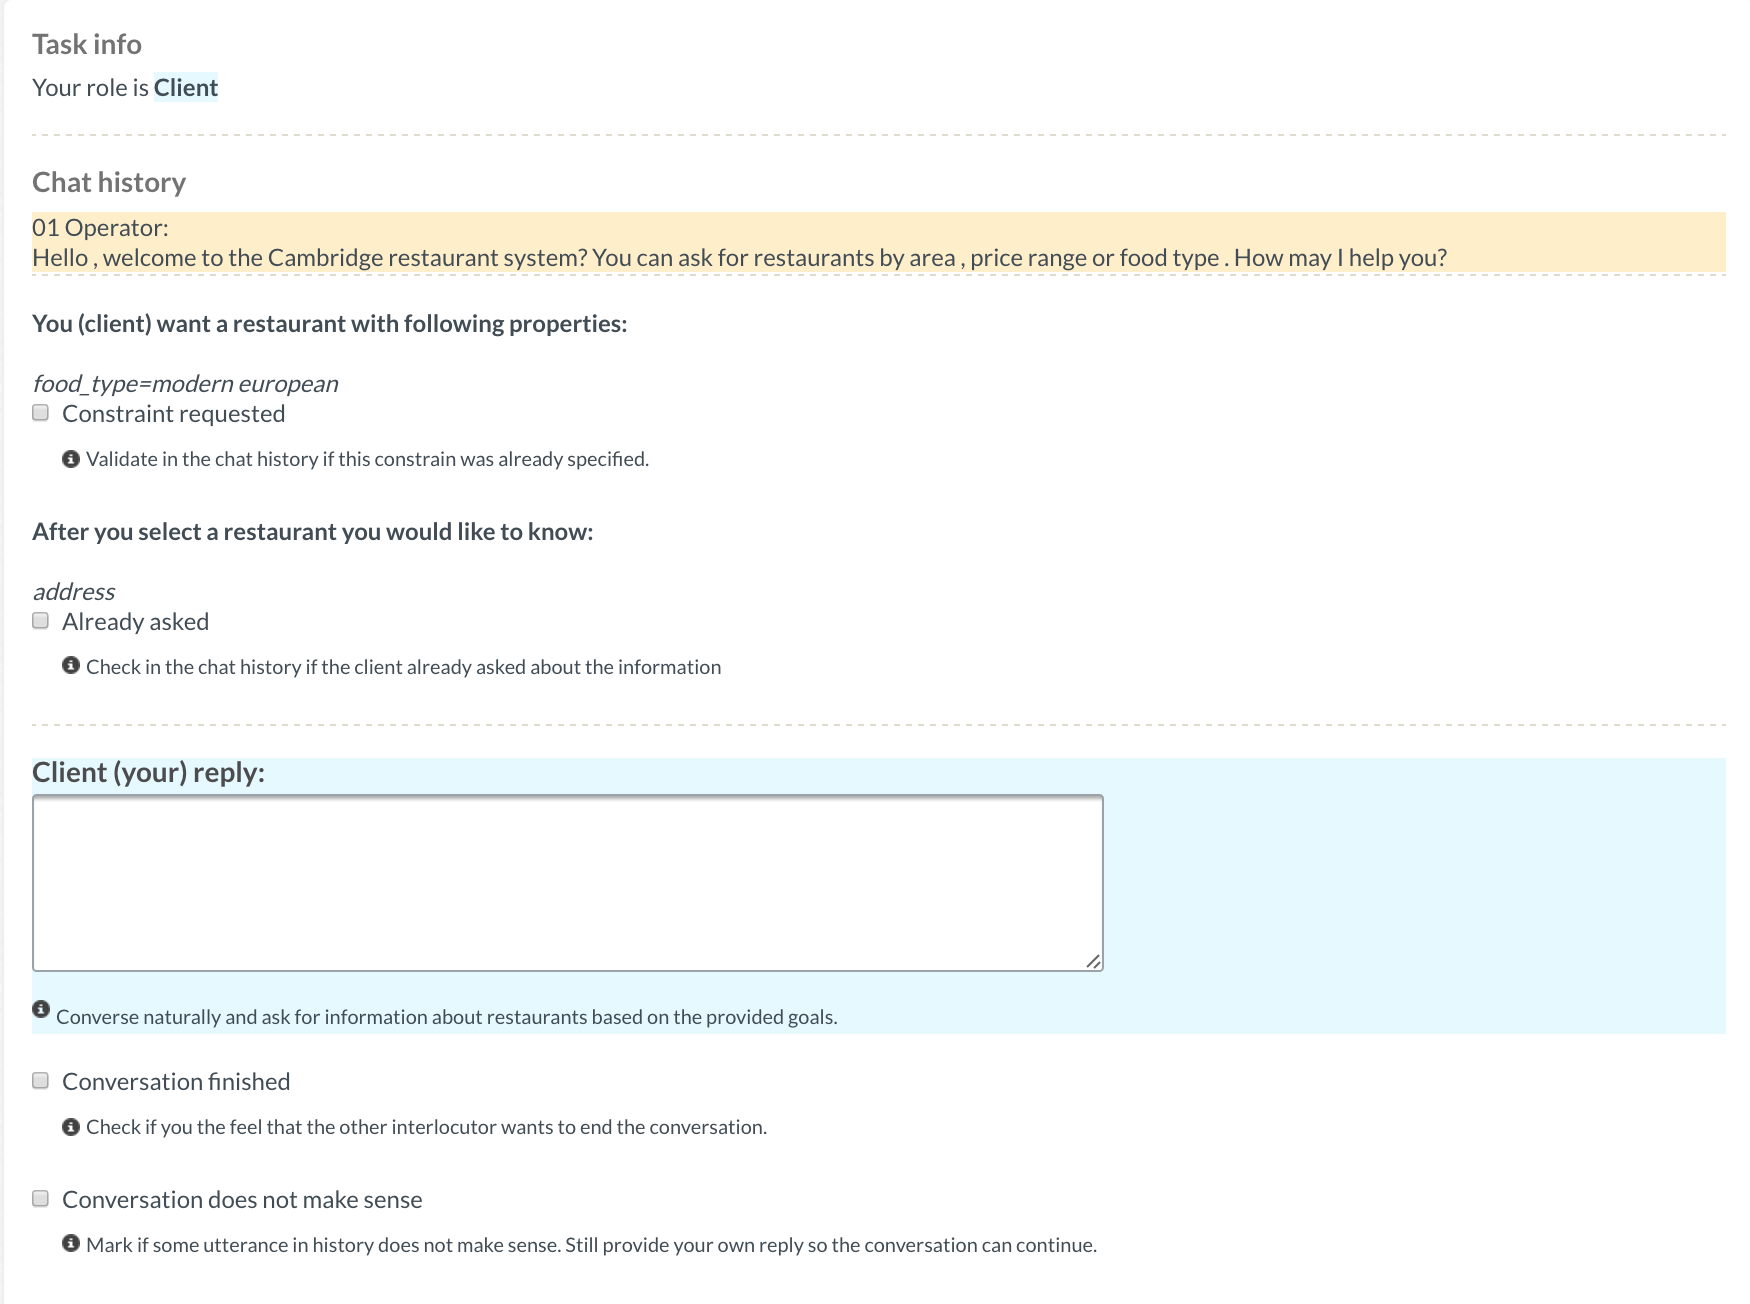
\includegraphics[height=30em]{gui-annotators-client}
\caption{Client annotation interface}
\end{center}
\vspace{-1.00em}
\label{fig:client}
\end{figure}
\vspace{-1.00em}

\vspace{-1.00em}
\subsection{Operator Interface}
\label{sec:operator}
The operator CF worker is asked to politely address the clients needs according to the information stored in the database.
In order to provide the information to clients, the operator uses the simple database interface depicted in~Figure~\ref{fig:operator}:
They filter the restaurants using a full text search over the database.
The~search interface is implemented in Javascript as a simple substring matching over values in the database.
We used such a simple interface because it is easy use for untrained CF workers.
Multiple constrains can be expressed by two substrings separated by a comma.
The content of the database is intentionally hidden if no filter is specified so that a filter has to be used to provide results.
The CF workers are also instructed to explicitly mark the database rows to which they refer in their answer.
Similarly to the client role, the operator does not have to provide all requested information in a single turn.
It is left up to the~worker which information is provided first.

\begin{figure}[tb]
\vspace{-1.00em}
\begin{center}
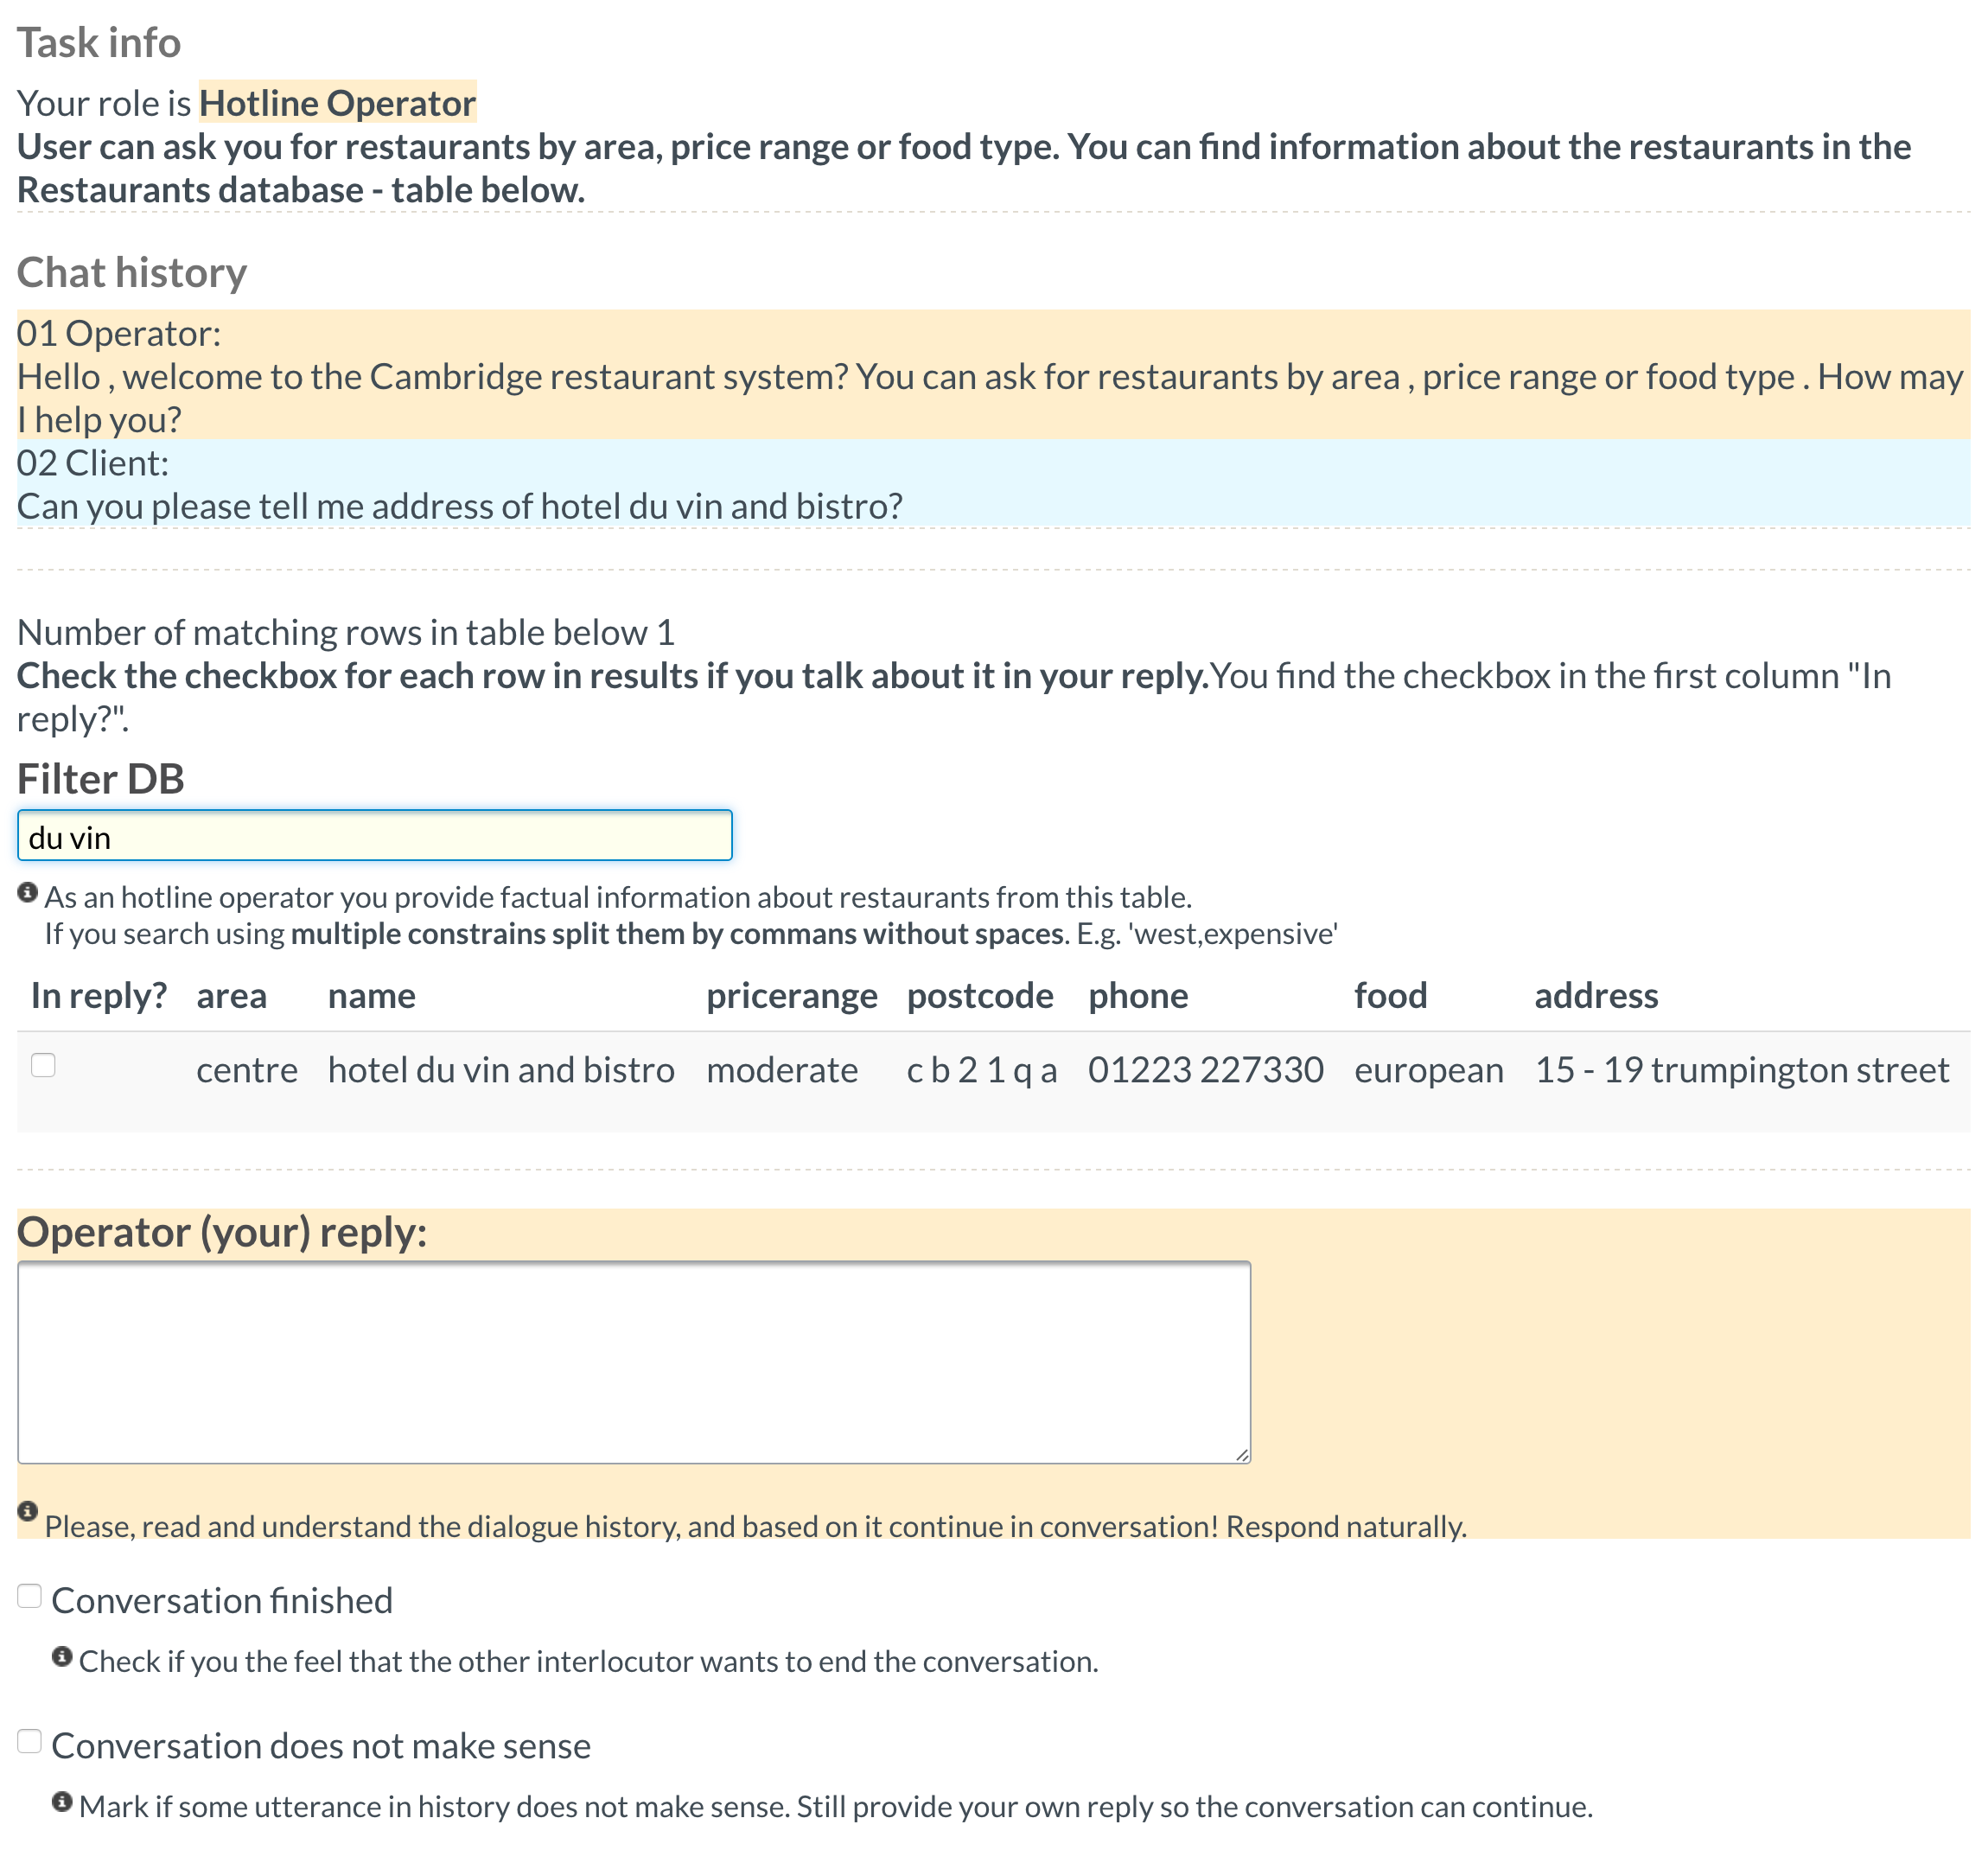
\includegraphics[height=35em]{gui-annotators-system}
\caption{Operator annotation interface}
\end{center}
\vspace{-1.00em}
\label{fig:operator}
\end{figure}
\vspace{-1.00em}

\vspace{-1.00em}
\subsection{Asynchronous collection without real-time responses}
\label{sec:async}
In this section, we describe how we combine the workers' replies to form a conversation.
We design the crowdsourcing jobs so that the CF contributors are able to work independently of each other.
The roles of client and operator take turns as partial conversations are submitted to CF for collecting a single new response.
As a consequence, a~single conversation is collected from multiple contributors over several job submissions.

Each utterance in the conversation may be submitted by a different contributor. Therefore, the contributors need to read carefully the dialogue history to understand the conversation before submitting their response.
The workers are able to mark dialogues which do not make sense and thus they self-assess the quality of the conversations.
The contributors mark the conversations as finished if they have no more goals to fulfill and all the goodbyes have been said.

We bootstrap the conversation either with an operator's introduction {\it ``Hello , welcome to the Cambridge restaurant system...''}, or we bootstrap the conversation with a~full turn where we add a client's greeting, e.g., {\it ``Hi''} to the operator's introduction.
If we initialize the dialogue with a~full turn, the first contributor plays role of the system. If we bootstrap the conversation only with~the operator's greeting, the first contributor plays the client's role.

In a~single CF task submission, we let the workers append a~single response to multiple different dialogues, taking on a random role in each of them.
The conversations are typically rather short circa four turns and therefore, full dialogues are collected after few rounds of submissions.
The workers are paid  the same amount of money for every submitted response regardless of whether they play the client or the operator role.

To avoid poor language level of English, we restricted the CF job to English-speaking countries.
We further perform heuristic checks for too trivial replies, and we enable the CF workers to rate each other's responses.
This help us filter low-quality conversations, but more importantly, it motivates the CF workers not to cheat.

\section{Dataset Properties} \label{sec:props}
\vspace{-0.50em}
We just started to collect our dataset and so far, we have only collected \OP{62} conversations.
The average length of a conversation is \OP{3.8} turns, meaning that the contributors in both roles reply in average circa three times before the conversation is finished\footnote{The first system utterance is automatically generated and for some conversations, the first client reply is also generated automatically, as described in Section~\ref{sec:async}}.
During an average conversation, \OP{2.4} goals are requested and \OP{1.9} answered.
There are two reason why there is more goals requested than answered.
We saw a rare case when the goal was actually answered, but was not left marked as unanswered.
However, much more common case is that the client asks for several goals e.g. phone and address, but he is satisfied if the operator provides just one of the goals e.g. phone. 
% Typically in \OP{65} \% case the conversation is ended by the client.
% As we mention the conversation are short, taking only from \OP{four to six turns} including first turn with greetings.
% \begin{table}
% \begin{center}
% \begin{tabular}{lrr}
% \hline
% Set   & \# Dialogues & \# Turns \\
% \hline
% % Joint  &  todo &  todo \\
% % /a/SSD/oplatek/e2end/log/2016-06-08-17-31-38.400-dstc-INDEP_labels-d0.7-w100-e100/
% % /a/SSD/oplatek/e2end/log/TEST-ORIGINAL-2016-06-08-17-31-38.400dstc-INDEP_labels-d0.7-w100-e100-reward-0.9080-step-0036224
% Train  &   ? & ? \\
% Dev &   ? & ? \\
% Test &   ? & ? \\
% \hline
% \end{tabular}
% \caption{Accuracy on development and test set}
% \vspace{-2em}
% \end{center}
% \label{tab:props}
% \end{table}
During the data collection process we discarded around \OP{35} \% of replies so far because the utterances were of low quality.
Note that we discard only the low-quality utterance; the prefix of the conversation is submitted for finishing the conversation in a next round of CF tasks.
Once we collect enough conversations, we intend to split them into training, development and test set. % (see Table~\ref{tab:props}).


\section{Related Work} \label{sec:related}
\vspace{-0.50em}
Our work is closely related  to work of~\cite{williams2013dstc1,henderson2014dstc2,henderson2014dstc3} in the sense that the conversation are held in the same domain.
On the other hand, the collection process differs substantially because we do not use any artificial system in the operator's role;
we rather focus on collecting high-quality human-human conversations. 
In addition, we do not collect complex LU and DST annotation in our work.

The~relevant work of~\cite{wen2016network} includes a collection of human-human dialogues in a domain similar to ours but more restricted.
Their dataset is not yet publicly available; therefore, we only compare to their statistics.
The dataset is of similar size as we intend to collect, and a~very similar collection scheme was used where Amazon Mechanical Turk workers submitted one reply at a time without being connected to each other in real-time.
On the other hand, they collected explicit dialogue state annotation, which takes a significant annotation effort.

Another line of research~\cite{vodolan2016data} used CF to collect human-human conversations for interactive learning dataset.
However, the collected dialogues were later annotated by expert annotators, which goes directly against our intentions to avoid any expensive annotation.

There is a~significant amount of work which used Wizard-of-Oz experiments~\cite{whittaker2002fish,walker1997evaluating,rieser2008learning} for studying linguistic properties of dialogues, evaluating proof-of-concept of a~dialogue system or even collecting bootstrap training data.
However, to our knowledge, no other work than~\cite{wen2016network} have used cheap crowdsourcing workers to collect a~full training dataset for supervised learning of dialogue management or end-to-end conversations.

\section{Conclusion and Future work} \label{sec:conc}
\vspace{-0.50em}
We present a new human-human dialogue dataset with annotation of user intention in the form of operator's database calls.
We also introduced a novel data collection setting which resembles work of operators in call centers and introduces minimum overhead to crowdsourcing workers.
The collected dialogues are published under Creative Commons 4.0 BY-SA license.\footnote{URL will be provided in the camera-ready version of the paper}  % lindat\footnote{todo where}.

We plan to increase the number of collected dialogues to 700 or more before the camera-ready deadline.
We intend to use the dataset to train and evaluate an~end-to-end conversational model which uses only operator's database calls as additional supervision to the recorded responses. 

% FIXME hidden for anonymised submission
% \vspace{-1.40em}
% \subsubsection*{Acknowledgments}
% We would like to thank Ondřej Dušek for useful comments.
% This research was partly funded by the Ministry of Education, Youth and Sports of the Czech Republic under the grant agreement LK11221, core research funding, grant GAUK 1915/2015, and also partially supported by SVV project number 260 333.
% It used language resources stored and distributed by the LINDAT/CLARIN project of the Ministry of Education, Youth and Sports of the Czech Repub- lic (project LM2015071).
% We gratefully acknowledge the support of NVIDIA Corporation with the donation of the Tesla K40c GPU used for this research.
% Cloud computational resources were provided by the MetaCentrum under the program LM2010005 and the CERIT-SC under the program Center CERIT Scientific Cloud, part of the Operational Program Research and Development for Innovations, Reg.\ no. CZ.1.05/3.2.00/08.0144.

% ``something in quotes'' using plain tex or use \enquote{the enquote command}.
% cref Demonstration: Cref at beginning of sentence, cref in all other cases.
%
% \Cref{fig:simple} shows a simple fact, although \cref{fig:simple} could also show something else.
%
% \Cref{tab:simple} shows a simple fact, although \cref{tab:simple} could also show something else.
%
% \Cref{sec:intro} shows a simple fact, although \cref{sec:intro} could also show something else.
%
% Brackets work as designed:
% <test>
%
% The symbol for powerset is now correct: $\powerset$ and not a Weierstrass p ($\wp$).
%
% \begin{inparaenum}
% \item All these items...
% \item ...appear in one line
% \item This is enabled by the paralist package.
% \end{inparaenum}
% In the bibliography, use \texttt{\textbackslash textsuperscript} for ``st'', ``nd'', ...:
% E.g., \enquote{The 2\textsuperscript{nd} conference on examples}.
% When you use \href{http://www.jabref.org}{JabRef}, you can use the clean up command to achieve that.


% Winery~\cite{Winery} is graphical \commentontext{modeling}{modeling with one \enquote{l}, because of AE} tool.
%%%%%%%%%%%%%%%%%%%%%%%%%%%%%%%%%%%%%%%%%%%%%%%%%%%%%%%%%%%%%%%%%%%%%%%%%%%%%%%
\vspace{-1.00em}
\bibliographystyle{splncs03}
\bibliography{paper}

% All links were last followed on June 28, 2016.
%%%%%%%%%%%%%%%%%%%%%%%%%%%%%%%%%%%%%%%%%%%%%%%%%%%%%%%%%%%%%%%%%%%%%%%%%%%%%%%

\end{document}
